\section{Introduction}

I've watched a lot of talks about agents. Speaker after speaker uses a different word for the same thing: the \emph{framework}, the \emph{scaffold}, the \emph{runtime}, the \emph{orchestration layer}, the \emph{harness}. But when they show how their system works, it's the same mechanism every time.

\begin{itemize}
\tightlist
\item
  A model is called.
\item
  Something decides what goes into the call.
\item
  Something acts on what comes back.
\item
  Something decides whether to go again.
\end{itemize}

The words don't line up. The mechanisms do.

That gap costs something:

\begin{itemize}
\tightlist
\item
  \textbf{Diagnosis.} If you can't name the parts of your agent, you can't say which part failed.
\item
  \textbf{Comparison.} You can't compare two systems whose authors describe them differently.
\item
  \textbf{The market.} The field keeps meeting the same few ideas as new products: memory layers, gateways, tool protocols, tracing platforms, sandboxes, evaluation suites. Without a map, it's hard to tell whether each is new or an old idea renamed.
\end{itemize}

The outer layer now has a name, \emph{harness engineering}, and evidence that it matters:

\begin{itemize}
\tightlist
\item
  Zhang et al.~\cite{zhang2026stop} argue that, among comparable frontier models, the harness can drive more of the variance in performance than the choice of model, so agents shouldn't be compared without disclosing their harness.
\item
  Fan et al.~\cite{fan2026empirical} hold a coding harness's loop fixed and vary three of its parts: planning, the action space and context management. Each one changes how the agent behaves.
\end{itemize}

Both treat the harness as what matters. Fan et al.~pick parts of a harness to vary. I ask what the complete set of parts is.

My answer is \textbf{reductive}: take an agent apart until the parts stop being shared across systems. It is also \textbf{mechanistic}: define each part by what it does on the path from a request to a response, not by what it's called or who sells it.

\textbf{Contributions.} The first three are the paper. The rest follow from them.

\begin{enumerate}
\def\labelenumi{\arabic{enumi}.}
\tightlist
\item
  \textbf{Agent = Harness(Model):} the model is a fixed function, and everything around it is harness (§2).
\item
  \textbf{Five primitives of a harness,} each defined by what it does and what it never does, with rules for the hard cases at their boundaries (§3--4).
\item
  \textbf{A build showing the five are enough:} a working agent, built one primitive at a time, where each step's missing piece is the next primitive (§5).
\item
  \textbf{Production hardening folds back} into the primitives instead of adding new ones (§6).
\item
  \textbf{A decomposition of three production harnesses,} Claude Code, Codex and opencode. Nothing needs a sixth primitive, and the study sharpens the rules (§7).
\item
  \textbf{A case study} in which the agent built here wrote much of the course that teaches it (§8).
\end{enumerate}

Everything here comes from an open course, \href{https://github.com/averagejoeslab/building-agents}{harness-engineering}. Every listing and every run I quote is there in full, with real output.

\section{Two primitives: the model and the harness}

Start with an agent and ask what it's made of. Two things.

\textbf{The model predicts.} Given tokens, it produces the tokens most likely to come next:

\begin{quote}
\textbf{TokensOut = Model(TokensIn)}
\end{quote}

From the outside, the model is a function. Between calls it has no memory. It can't read a terminal or run a command. It can't decide to be called again. All it knows about this moment is in the tokens it's handed. Building it is \emph{model development}: training data, compute, and the methods to train and evaluate a model. That's its own discipline, and I treat what it produces as fixed.

\textbf{The harness does everything else.} It decides:

\begin{itemize}
\tightlist
\item
  how inputs are gathered;
\item
  how they're presented to the model;
\item
  how the model is called;
\item
  how its outputs are handled;
\item
  how information flows between all of them.
\end{itemize}

\begin{quote}
\textbf{Agent = Harness(Model)}
\end{quote}

The model goes inside, and the harness wraps it. Harness engineering is building that second part.

The split is blunt on purpose. Anything that isn't the model's weights is harness: a system prompt, a tool, a retry policy, a memory store. Two agents on the same model differ only in their harnesses, so a comparison that leaves out the harness is comparing the wrong thing.

\subsection{Method}

The method is one question:

\begin{quote}
\emph{What is it, and by what mechanistic primitives does it work?}
\end{quote}

Asking it gives a sequence of answers:

\begin{enumerate}
\def\labelenumi{\arabic{enumi}.}
\tightlist
\item
  \textbf{Ask it of an agent} and you get a model and a harness.
\item
  \textbf{Ask it of a harness} and you get five primitives (§3).
\item
  \textbf{Ask it once more,} of a primitive, and the answers stop being shared. One harness's input reads a terminal, another's reads a Slack channel, and a third's reads a webhook.
\end{enumerate}

That's where taking apart ends. A primitive is the deepest level at which every harness still has the same parts.

Each primitive gets two definitions:

\begin{itemize}
\tightlist
\item
  \textbf{positive:} what it does;
\item
  \textbf{negative:} what it never does, naming which other primitive owns that job.
\end{itemize}

The negative definitions do most of the work. They make the primitives disjoint, so every piece of harness code has exactly one home. A piece is placed by \textbf{what it does, not where the code sits} or what it's called (§4).

\subsection{Scope}

The primitives describe what happens on the path of a request at run time. Some of what ships with a harness never runs on that path, and I leave it out of scope the way I leave out model development:

\begin{itemize}
\tightlist
\item
  \textbf{Transport and hosting:} a client/server split, a remote workspace, the process that serves the UI.
\item
  \textbf{Persistence:} the database.
\item
  \textbf{Event wiring:} an internal event bus.
\item
  \textbf{Configuration and packaging:} loading settings, installing plugins.
\end{itemize}

They carry, store or configure the primitives without being a step in a pass. Where they do something on the path, such as a saved transcript the harness replays, that piece is placed like any other.

\section{The five primitives}

\begin{figure}[t]
\centering
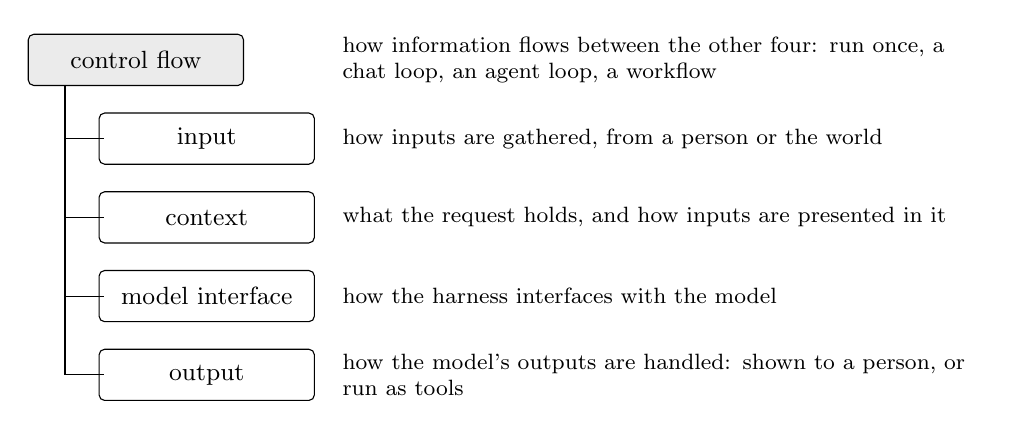
\begin{tikzpicture}[
  box/.style={draw, rounded corners=2pt, minimum height=6.5mm, text width=25mm, align=center, font=\small},
  note/.style={font=\footnotesize, text width=80mm, align=left, anchor=west}]
\node[box, fill=black!8] (cf) at (0,0) {control flow};
\node[note] at (2.5,0) {how information flows between the other four: run once, a chat loop, an agent loop, a workflow};
\foreach \y/\name/\txt in {-1/input/{how inputs are gathered, from a person or the world},
                           -2/context/{what the request holds, and how inputs are presented in it},
                           -3/model interface/{how the harness interfaces with the model},
                           -4/output/{how the model's outputs are handled: shown to a person, or run as tools}} {
  \node[box] at (0.9,\y) {\name};
  \node[note] at (2.5,\y) {\txt};
  \draw (-0.9,\y) -- (-0.4,\y);
}
\draw (-0.9,-0.33) -- (-0.9,-4);
\end{tikzpicture}
\caption{The five primitives of a harness. Control flow wraps the other four.}
\label{fig:tree}
\end{figure}


One pass through a harness follows one path:

\begin{figure}[t]
\centering
\begin{tikzpicture}[
  node distance=3.5mm,
  prim/.style={draw, rounded corners=2pt, minimum height=8mm, align=center, font=\footnotesize, fill=black!6},
  data/.style={font=\footnotesize\itshape, align=center},
  >=Latex]
\node[data] (pw) {person\\or world};
\node[prim, right=of pw] (in) {input};
\node[prim, right=of in] (ctx) {context};
\node[data, right=of ctx] (req) {request};
\node[prim, right=of req] (mi) {model\\interface};
\node[data, right=of mi] (resp) {response};
\node[prim, right=of resp] (out) {output};
\node[data, right=of out] (pw2) {person\\or world};
\draw[->] (pw) -- (in); \draw[->] (in) -- (ctx); \draw[->] (ctx) -- (req);
\draw[->] (req) -- (mi); \draw[->] (mi) -- (resp); \draw[->] (resp) -- (out); \draw[->] (out) -- (pw2);
\draw[->] (out.south) -- ++(0,-6mm) -| node[pos=0.25, below, font=\footnotesize\itshape] {result} (in.south);
\end{tikzpicture}
\caption{One pass through a harness. A tool's result comes back as input; control flow decides whether to go around again.}
\label{fig:path}
\end{figure}


\begin{enumerate}
\def\labelenumi{\arabic{enumi}.}
\tightlist
\item
  Input gathers what goes in.
\item
  Context assembles it into a request and makes it fit.
\item
  The model interface sends the request and gets the response.
\item
  Output handles the response, by showing it to a person or running a tool. A tool's result comes back as input.
\item
  Control flow decides what happens at the end: go around again, give a person a turn, or stop.
\end{enumerate}

\subsection{Model interface}

\textbf{Does:} sends tokens to the model as a request and gets tokens back as a response.

\textbf{Never does:} decide when to call (control flow), gather what goes in (input), decide how it's presented (context), or act on what comes back (output).

It's the thinnest primitive, because of where it sits. The other four live on the harness's side. The model interface is the boundary: in \emph{Agent = Harness(Model)}, it's the parentheses. At its smallest it's one SDK call. Bigger ones vary along a few lines:

\begin{itemize}
\tightlist
\item
  \textbf{Where the request goes:} a hosted API, a local model, a gateway.
\item
  \textbf{How it travels:} an SDK, raw HTTP, a layer that translates between providers.
\item
  \textbf{Which model answers:} one model, or a backup for when the first is down.
\item
  \textbf{How the response arrives:} all at once, or streamed.
\item
  \textbf{How many requests go:} one at a time, or a batch.
\item
  \textbf{What happens when a request fails:} retry, wait, time out.
\item
  \textbf{The request's settings:} output cap, thinking effort, whether you get a summary of the thinking.
\end{itemize}

All of it is about getting one request there and one response back.

\subsection{Input}

\textbf{Does:} gathers what goes to the model, from a \textbf{person} (a task, a question, a message) or from \textbf{the world} (what happened when a tool ran: what it printed, its exit code, whether it failed).

\textbf{Never does:} decide how what it gathered is laid out in the request (context), send it (model interface), or decide whether to go again (control flow).

Input is the harness's afferent pathway, carrying signals in.

\begin{itemize}
\tightlist
\item
  \textbf{Where it comes from:} command-line arguments, a prompt, a pipe, a chat app, a webhook, a schedule.
\item
  \textbf{What it can be:} text, images, files.
\end{itemize}

Wherever it comes from, input does one thing: it brings something from outside the harness to the edge of the request.

\subsection{Output}

\textbf{Does:} handles the model's response, by \textbf{showing it} to a person or \textbf{running it} as a tool.

\textbf{Never does:} decide whether a tool's result goes back to the model (control flow), or what the next request holds (context).

Output is the efferent pathway, carrying actions out. The model can't act, but it can ask. Its response can include a request to use a tool: a name and arguments, in a shape the harness described to it. Output runs the request, and what happened comes back as input. \textbf{The model asks; the harness acts.} Output's choices include:

\begin{itemize}
\tightlist
\item
  \textbf{Which tools exist:} one general tool, or many specific ones.
\item
  \textbf{Where they run:} this machine, a container, a remote host, the provider.
\item
  \textbf{How they run:} one after another, or at the same time.
\item
  \textbf{When not to run:} a request cut off mid-generation is incomplete, and running half a command is worse than running none.
\item
  \textbf{What happens when a tool fails or hangs.}
\end{itemize}

Input and output are built separately, but they're two ends of one exchange, and they meet at the tool. A tool needs both: output to run it, and input to bring back what happened.

\subsection{Control flow}

\textbf{Does:} \textbf{sequences} the other four, passing what one produced to the next, and \textbf{terminates}, deciding when to stop or hand back to a person.

\textbf{Never does:} send the request (model interface), gather (input), present (context), or handle the response (output).

Control flow is the one primitive that wraps the others. How it arranges them decides what you've built:

{\def\LTcaptype{none} % do not increment counter
\begin{longtable}[]{@{}
  >{\raggedright\arraybackslash}p{(\linewidth - 4\tabcolsep) * \real{0.3333}}
  >{\raggedright\arraybackslash}p{(\linewidth - 4\tabcolsep) * \real{0.3333}}
  >{\raggedright\arraybackslash}p{(\linewidth - 4\tabcolsep) * \real{0.3333}}@{}}
\toprule\noalign{}
\begin{minipage}[b]{\linewidth}\raggedright
Shape
\end{minipage} & \begin{minipage}[b]{\linewidth}\raggedright
Arrangement
\end{minipage} & \begin{minipage}[b]{\linewidth}\raggedright
Who decides what happens next
\end{minipage} \\
\midrule\noalign{}
\endhead
\bottomrule\noalign{}
\endlastfoot
Single call & input \(\rightarrow\) call \(\rightarrow\) output, stop & nobody; it's fixed \\
Chat loop & call, show, hand back to the person, repeat & the person \\
Workflow & your code lays out the calls: draft, judge, rewrite & your code \\
Agent loop & call; while the model asks for tools, run them, send the results back, call again & the model \\
\end{longtable}
}

So the line between a \emph{workflow} and an \emph{agent} \cite{schluntz2024building} is a fact about control flow: who decides the next step. Termination is half the definition, not an afterthought. A loop with no clear way to end is a bill with no clear way to end. The smallest agent loop ends when the model stops asking for tools. Bigger ones also stop on a step limit, a spending limit, a refusal, or a person saying stop.

\subsection{Context}

\textbf{Does:} before every call, \textbf{assembles} what the request holds and \textbf{fits} it into the space the model can read.

\textbf{Never does:} gather inputs (input), send the request (model interface), or decide when to call (control flow).

Every call starts from nothing. The model doesn't know where it's running, what day it is, who it is, what it did a minute ago, or what you told it last week, unless the harness puts it in the request. That's why so much of what people build into harnesses turns out to be context. These components are all ways of deciding what the model sees:

\begin{itemize}
\tightlist
\item
  \textbf{instructions:} the system prompt;
\item
  \textbf{working memory:} this session;
\item
  \textbf{episodic memory:} past sessions;
\item
  \textbf{semantic memory:} facts that last;
\item
  \textbf{procedural memory:} skills, recipes, playbooks;
\item
  \textbf{retrieval:} search results put in the request;
\item
  \textbf{compaction:} a summary in place of history that no longer fits;
\item
  \textbf{self-knowledge:} the agent's own description, or its own source.
\end{itemize}

Input and context aren't the same thing. Input brings something to the edge of the request. Context decides whether it goes in, where, in what form, and what gets dropped to make room.

\subsection{Summary}

{\def\LTcaptype{none} % do not increment counter
\begin{longtable}[]{@{}
  >{\raggedright\arraybackslash}p{(\linewidth - 4\tabcolsep) * \real{0.3333}}
  >{\raggedright\arraybackslash}p{(\linewidth - 4\tabcolsep) * \real{0.3333}}
  >{\raggedright\arraybackslash}p{(\linewidth - 4\tabcolsep) * \real{0.3333}}@{}}
\toprule\noalign{}
\begin{minipage}[b]{\linewidth}\raggedright
Primitive
\end{minipage} & \begin{minipage}[b]{\linewidth}\raggedright
Does
\end{minipage} & \begin{minipage}[b]{\linewidth}\raggedright
Never does
\end{minipage} \\
\midrule\noalign{}
\endhead
\bottomrule\noalign{}
\endlastfoot
Model interface & request out, response back & decide when, gather, present, act \\
Input & gather from a person or the world & present, send, decide to go again \\
Output & show the response, or run a tool & decide whether results return, shape the next request \\
Control flow & sequence and terminate & send, gather, present, handle \\
Context & assemble and fit the request & gather, send, decide when \\
\end{longtable}
}

\section{Rules for the hard cases}

A taxonomy is only as good as its hard cases. The rules below settle the ones that come up. Each follows from the negative definitions in §3. Several were sharpened by the decomposition study in §7, and I mark those.

\textbf{Place by what it does, not where it lives.} Code that decides what the model sees is context, even inside a tool. Examples:

\begin{itemize}
\tightlist
\item
  opencode attaches nested AGENTS.md files to the Read tool's result;
\item
  Claude Code's WebFetch runs a separate model call to shrink a page before the model sees it.
\end{itemize}

A guardrail decision is control flow even when it runs inside a tool's execution, as Codex's approval routine does. \emph{(Sharpened by §7.)}

\textbf{``Is a tool'' doesn't mean ``is output.''} In all three production harnesses, the model drives other primitives through tool calls: spawning a subagent, entering plan mode, writing a task list, searching for tools, scheduling a wake-up, asking for a new context window. The tool call is output. Its effect lands on the primitive it changes: control flow, context or input. \emph{(From §7.)}

\textbf{Backup or routing: ask what triggered the switch.}

\begin{itemize}
\tightlist
\item
  \textbf{The request couldn't be served} by the first model, because it was down, overloaded, or refused the request: switching to another model is the \textbf{model interface}. It only changes how one request gets a response.
\item
  \textbf{The switch is keyed to the work:} this task is simple, this phase is planning. That's \textbf{routing}, which is \textbf{control flow}, because it's a decision about the work.
\end{itemize}

Some cases to check the rule against:

\begin{itemize}
\tightlist
\item
  \emph{A fixed model for one kind of request,} such as compaction summaries, is a request setting. That's the model interface.
\item
  \emph{Claude Code's \passthrough{\lstinline!opusplan!}} uses one model to plan and another to execute. It's keyed to the phase, so it's control flow.
\item
  \emph{A content-classifier fallback} that retries a flagged request on another model is the model interface. Keeping the second model for the rest of the session is a separate, control-flow decision.
\end{itemize}

\emph{(Sharpened by §7.)}

\textbf{Streaming.} \emph{Receiving} a response as a stream is the model interface. \emph{Printing} each piece as it arrives is output.

\textbf{Parallelism.} Running several \emph{tool requests} from one response at once is output: it's how those requests get executed. Making several \emph{model calls} at once, to fan out subtasks or to vote, is a way of arranging the work, so it's control flow.

\textbf{Who reads it.}

\begin{itemize}
\tightlist
\item
  Something kept \textbf{for the model}, such as an episode log the agent can search later, is \textbf{context}.
\item
  Something kept \textbf{for the operator}, such as a trace of every call, is \textbf{observability} (§6).
\item
  Something made \textbf{for the user}, such as a per-turn diff of changed files, is \textbf{output}: showing to a person.
\end{itemize}

The same file can serve two readers. Claude Code's session transcript is read by the operator and replayed by the harness on resume. In that case each use is placed separately. \emph{(Sharpened by §7.)}

\textbf{Who uses a person's answer.}

\begin{itemize}
\tightlist
\item
  When the \textbf{harness} consumes the answer, as with ``allow this command? {[}y/N{]}'', it's a \textbf{control-flow} decision, not new input.
\item
  When the \textbf{model} consumes it, as when the model asks the person a question and gets the answer back as a tool result, it's \textbf{input} from a person.
\end{itemize}

\emph{(From §7: Codex's \passthrough{\lstinline!request\_user\_input!}, opencode's question tool, Claude Code's AskUserQuestion.)}

\textbf{A person acting directly.} A shell command the \emph{person} runs, such as \passthrough{\lstinline"!cmd"} in Codex, Claude Code and opencode, brings world state into the conversation. That's input, even though it reuses output's executor. \emph{(From §7.)}

\textbf{Programs the model writes.} If the program sequences \emph{model calls}, it's control flow, written at run time. Claude Code's workflow scripts are the example. If it only sequences \emph{tools}, it's output: a script, however clever. The code modes in Codex and opencode run model-written JavaScript that calls tools without calling the model, so today they're output. \emph{(From §7.)}

\textbf{Bundles aren't parts.} A \emph{mode}, a \emph{skill}, a \emph{hook system} or an \emph{agent profile} is packaging. Each bundles settings across several primitives. Split it and every piece lands in one:

\begin{itemize}
\tightlist
\item
  Plan mode is a context template, plus tools removed, plus an approval gate.
\item
  A skill is procedural memory, plus scripts the model can run, plus a tool allow-list.
\item
  A hook system is a dispatcher (control flow) whose events each touch one primitive.
\end{itemize}

\emph{(From §7.)}

\textbf{The ``augmented LLM.''} The building block of a model with retrieval, tools and memory \cite{schluntz2024building} isn't a primitive. It splits into context (retrieval, memory) and output (tools) around a model interface.

\textbf{Tool protocols.} MCP \cite{mcp} is mostly output you plug in: tools someone else built, behind one protocol. Its other features land elsewhere:

\begin{itemize}
\tightlist
\item
  resources and prompts decide what the model sees, so they're \textbf{context};
\item
  \emph{sampling} borrows the client's \textbf{model interface};
\item
  \emph{elicitation} asks the person, which is \textbf{input}.
\end{itemize}

\emph{(Sharpened by §7.)}

\textbf{Multiple agents.} One agent handing a task to another is a shape of control flow: the outer harness sequencing an inner one. Delegation adds no new primitive. It nests harnesses. The same rule covers model-backed parts \emph{inside} a harness: an approval reviewer, a stop judge, a memory extractor. Each is control flow plus a model-interface call.

\section{Building it back up: the five are enough}

A taxonomy can be complete on paper and still miss something in practice. The test is to build an agent from nothing but the five and see whether anything else is needed. That's the heart of the course, its first four lessons, and the heart of this paper.

The build goes outward from the model, in a different order from §3:

\begin{itemize}
\tightlist
\item
  the model interface comes first, because nothing reaches the model without it;
\item
  each later step adds the primitive the last one was missing.
\end{itemize}

The example is quark, my own agent. Each lesson's \passthrough{\lstinline!quark.py!} is the last lesson's file plus that primitive and nothing else. It's one way to build each primitive, not the only way.

\subsection{The model interface alone (9 lines)}

The first harness is one call. It sends a hard-coded question, \emph{``What's in this directory?''}, and prints the whole response. The response has three fields that matter:

\begin{itemize}
\tightlist
\item
  \passthrough{\lstinline!content!}: the tokens out, as blocks;
\item
  \passthrough{\lstinline!stop\_reason!}: why it stopped;
\item
  \passthrough{\lstinline!usage!}: tokens in and out.
\end{itemize}

The reply is the lesson. The model says it can't see the directory and suggests running \passthrough{\lstinline!ls!}. \textbf{It knows the right next step and can't take it.} Both ends are stubs: the input is a string no one typed, and the output is a dump that handles nothing.

\subsection{Input and output (21 lines)}

Input and output are built separately, then put together.

\begin{itemize}
\tightlist
\item
  \textbf{Input} takes a task from the command line and describes one tool, \passthrough{\lstinline!bash!}, in the request. Given \emph{``how many lines are in README.md?''}, the model answers the only way it can: a \passthrough{\lstinline!tool\_use!} block asking for \passthrough{\lstinline!wc -l README.md!}, with \passthrough{\lstinline!stop\_reason: tool\_use!}. Output is still a stub, so nothing runs it. The model asked; nothing acted.
\item
  \textbf{Output} handles each block of the response. It prints text, and it runs a tool request with \passthrough{\lstinline!subprocess!}.
\item
  \textbf{Together} they need one more piece neither had alone: the command's result, wrapped as a \passthrough{\lstinline!tool\_result!}. That's input from the world.
\end{itemize}

The joined harness runs \passthrough{\lstinline!wc -l!} and prints \passthrough{\lstinline!71 README.md!}. \textbf{The model never sees the 71.} It sits in a list, and nothing sends it. The path ends at output.

\subsection{Control flow (30 lines)}

Lesson 2 goes inside \passthrough{\lstinline!while True!}. The response and the results are appended to \passthrough{\lstinline!messages!}. If the model asked for anything, the loop calls again. When it stops asking, the run ends, or, in a chat, it hands back to you.

Asked which lesson's \passthrough{\lstinline!quark.py!} is longest, the agent ran one \passthrough{\lstinline!find … | wc -l!} and answered from what it found. That's two calls, and the second only happened because the first one's result went back.

That's an agent now: the model decides what happens next. The same four pieces, arranged differently, make a single call, a chatbot or a workflow (§3.4). The lesson's second example is a workflow, an evaluator--optimizer, where your code decides the order of the calls.

\textbf{But it knows nothing:} not where it is, not what day it is, not who it is, not what you told it yesterday. And \passthrough{\lstinline!messages!} grows every pass, so a long session will outgrow what the model can read. Something has to decide what the model sees.

\subsection{Context (48 lines)}

The last primitive adds five context components:

\begin{itemize}
\tightlist
\item
  \textbf{Working memory.} Lesson 3's \passthrough{\lstinline!messages!}, renamed for what it is.
\item
  \textbf{Instructions.} A system prompt written as models of self, world, other selves and body. It's rebuilt every call, so the directory and the date are current.
\item
  \textbf{Self-knowledge.} quark's own source file, put in that prompt so the model can see the harness it runs in.
\item
  \textbf{Semantic memory.} A file the agent reads and writes with the tool it already has. There's no memory code at all.
\item
  \textbf{Reactive compaction.} When the API refuses a request as too long, the oldest turns are dropped and the rest summarized.
\end{itemize}

The runs show it working:

\begin{enumerate}
\def\labelenumi{\arabic{enumi}.}
\tightlist
\item
  \textbf{Asked what it is,} quark describes its name, its body, its loop and its memory file, because they're in its context.
\item
  \textbf{Told \emph{``remember that I prefer short answers''},} it writes that to its memory file.
\item
  \textbf{In a new session,} with empty working memory, asked what it knows about me, it reads the file and answers.
\end{enumerate}

Working memory carried nothing between the runs. Semantic memory did.

\subsection{What the build shows}

{\def\LTcaptype{none} % do not increment counter
\begin{longtable}[]{@{}
  >{\raggedright\arraybackslash}p{(\linewidth - 6\tabcolsep) * \real{0.2500}}
  >{\raggedright\arraybackslash}p{(\linewidth - 6\tabcolsep) * \real{0.2500}}
  >{\raggedright\arraybackslash}p{(\linewidth - 6\tabcolsep) * \real{0.2500}}
  >{\raggedright\arraybackslash}p{(\linewidth - 6\tabcolsep) * \real{0.2500}}@{}}
\toprule\noalign{}
\begin{minipage}[b]{\linewidth}\raggedright
Step
\end{minipage} & \begin{minipage}[b]{\linewidth}\raggedright
Adds
\end{minipage} & \begin{minipage}[b]{\linewidth}\raggedright
\passthrough{\lstinline!quark.py!}
\end{minipage} & \begin{minipage}[b]{\linewidth}\raggedright
What's still missing
\end{minipage} \\
\midrule\noalign{}
\endhead
\bottomrule\noalign{}
\endlastfoot
1 & Model interface & 9 lines & Both ends are stubs. The model says the next step is \passthrough{\lstinline!ls!}, and nothing can run it. \\
2 & Input and output & 21 lines & A tool runs, but its result never reaches the model. \\
3 & Control flow & 30 lines & The result goes back, but the agent knows nothing about itself, its world or its past, and its history grows without limit. \\
4 & Context & 48 lines & Nothing. It works, remembers, knows what it is, and compacts when it's full. \\
\end{longtable}
}

Each step's missing piece is the next primitive, and no step needs anything outside the five. The finished harness is in Appendix A.

Each primitive also gets a fuller second example, to show that a primitive is a space of choices, not one design:

\begin{itemize}
\tightlist
\item
  \textbf{Model interface:} timeouts, retries, a backup model, streaming and adjustable thinking.
\item
  \textbf{Input and output:} input and output through a Telegram chat, with two tools run at the same time, timeouts, and an incomplete request that isn't run.
\item
  \textbf{Control flow:} a step limit and refusal handling, plus the evaluator--optimizer workflow.
\item
  \textbf{Context:} an episode log, skill files, token counting before each call, and trimming of long tool results.
\end{itemize}

None of them needed a sixth primitive.

\section{Production hardening folds back into the primitives}

A harness that works isn't one you'd run unattended. Production agents add tracing, approvals, sandboxes, retries, caching and evaluation. Each has its own vendors and its own literature, so it's natural to treat each one as a new building block. The primitives say otherwise:

\begin{quote}
\textbf{Corollary.} Production concerns add \emph{hardening}, not new primitives. Each piece of a production layer lands inside a primitive, where that primitive already acts.
\end{quote}

The course's second part tests this one layer at a time:

\begin{itemize}
\tightlist
\item
  Each production lesson's \passthrough{\lstinline!quark.py!} is the previous one plus that layer.
\item
  Each names the primitives it's built on.
\item
  Each ends with a \emph{``Notice what {[}layer{]} never does''} paragraph naming the primitives it leaves alone.
\end{itemize}

{\def\LTcaptype{none} % do not increment counter
\begin{longtable}[]{@{}
  >{\raggedright\arraybackslash}p{(\linewidth - 8\tabcolsep) * \real{0.1333}}
  >{\raggedright\arraybackslash}p{(\linewidth - 8\tabcolsep) * \real{0.1333}}
  >{\raggedright\arraybackslash}p{(\linewidth - 8\tabcolsep) * \real{0.2000}}
  >{\raggedright\arraybackslash}p{(\linewidth - 8\tabcolsep) * \real{0.4000}}
  >{\raggedright\arraybackslash}p{(\linewidth - 8\tabcolsep) * \real{0.1333}}@{}}
\toprule\noalign{}
\begin{minipage}[b]{\linewidth}\raggedright
Layer
\end{minipage} & \begin{minipage}[b]{\linewidth}\raggedright
Folds into
\end{minipage} & \begin{minipage}[b]{\linewidth}\raggedright
Why there
\end{minipage} & \begin{minipage}[b]{\linewidth}\raggedright
Mechanism
\end{minipage} & \begin{minipage}[b]{\linewidth}\raggedright
Lines added (\passthrough{\lstinline!quark.py!})
\end{minipage} \\
\midrule\noalign{}
\endhead
\bottomrule\noalign{}
\endlastfoot
Observability & control flow & the only primitive that sees the whole sequence & read the clock, \passthrough{\lstinline!usage!} and exit codes that are already there; append one JSON line per event & +12 (59) \\
Guardrails & control flow (mostly) & control flow already decides whether a request becomes a command, and whether to go again & allow, ask or deny before each tool; a refusal returned as a readable tool result; step, token, cost and repeat limits; an interrupt & +26 (83) \\
Sandboxing & output & \emph{where} a tool runs was always output's choice & commands run by \passthrough{\lstinline!docker exec!} in a container with no network, capped resources, a read-only root and only the working folder mounted, so the kernel enforces the limits, not a check on the text & +13 (94) \\
Resilience & model interface, output, context & where the world can say no, and what must be replayed & retry transient failures with backoff, fall back to a backup model, stop cleanly; answer every tool request even when it's broken; save each step and resume, marking an interrupted command as \emph{may or may not have run} & +53 (135) \\
Performance & context, model interface, output & where the tokens and the waiting are & cache marks and trimming (context); streaming and a fixed small model for summaries (model interface); tools run at the same time (output) & +47 (159) \\
Evaluation & outside the harness & it treats the agent as a box & an outer loop that sets up a case, runs the real agent, grades what it left behind, and compares with the last run & +38 (196) \\
\end{longtable}
}

A few rows need more than a table cell.

\textbf{Some layers span several primitives without adding one.}

\begin{itemize}
\tightlist
\item
  \textbf{Resilience.} A retry happens inside one call, so it's the model interface. Answering a broken tool request is output. Resuming a run replays saved working memory, which is context. Codex does the same at request-assembly time: it fills in ``aborted'' results for tool calls that never finished.
\item
  \textbf{Performance.} Running the model's tool requests together is output. A cache mark is a choice about how the request is laid out, so it's context. Performance's fuller example also routes each task to a model tier, and that part is control flow, by the routing rule in §4.
\end{itemize}

\textbf{Guardrails mostly sit in control flow, but not entirely.} In opencode and Claude Code, denied tools are also removed from the request, and that slice is context. The decision still has one home; the enforcement can reach into another primitive.

\textbf{Layers aren't independent of each other.} I first wrote that each layer ``leaves the other primitives unchanged.'' The production harnesses show that's too strong. In Codex, the approval policy and the sandbox policy feed each other:

\begin{enumerate}
\def\labelenumi{\arabic{enumi}.}
\tightlist
\item
  The approval requirement is computed from the sandbox setting.
\item
  An approval changes how the command runs.
\item
  A sandbox denial triggers a new approval.
\end{enumerate}

Claude Code is the same: its sandbox can stand in for a permission prompt, and the model can ask to leave the sandbox, which sends that request back through the guardrails. Each piece still lands in one primitive. What the study shows is that layers can read each other's state. The primitives stay disjoint; the layers don't stay separate.

\textbf{Evaluation is the exception that proves the rule.} It sits in none of the five, because it stands outside the agent. But it's built \emph{from} them:

\begin{itemize}
\tightlist
\item
  an outer \textbf{control-flow} loop;
\item
  the task handed in as \textbf{input};
\item
  the check run as \textbf{output};
\item
  a model grader reached through the \textbf{model interface}.
\end{itemize}

It's a second harness wrapped around the first. In the course it caught a change that looked harmless. Lowering the step limit from 20 to 1 kept three of four cases passing and flagged the fourth as \passthrough{\lstinline!REGRESSED!}. In the production harnesses, evaluation is just as clearly outside:

\begin{itemize}
\tightlist
\item
  \textbf{Codex and opencode} ship only engineering tests, against a mocked or recorded model.
\item
  \textbf{Claude Code's} \passthrough{\lstinline!claude plugin eval!} grades plugins and skills by running the real agent.
\end{itemize}

So the production harness of 196 lines reads under the same five headings as the 48-line one. The layers make the primitives sturdier; they don't add to them. I show the corollary by cases, not by proof, and §9 says what would refute it.

\section{Taking apart production harnesses}

If the primitives are right, real harnesses should sort under them, including big ones that weren't written to teach anything. I took apart three production coding agents, part by part, with the checklist the course ends on:

\begin{lstlisting}
control flow          what kind of loop? who decides when to stop?
├── input             where do inputs come from: people, the world, both?
├── context           what does the request hold? which memories? how does it fit?
├── model interface   where does the request go, and how does the response come back?
└── output            where do outputs go? which tools, and how are they run?
\end{lstlisting}

\subsection{Method}

For each harness:

\begin{enumerate}
\def\labelenumi{\arabic{enumi}.}
\tightlist
\item
  I mapped the modules on the request path.
\item
  I assigned every meaningful part to exactly one primitive, or to a production layer with the primitive it folds into, with evidence and a reason from the definitions in §3.
\item
  I listed every part that was hard to place, and asked of each: does it fit none of the five?
\end{enumerate}

{\def\LTcaptype{none} % do not increment counter
\begin{longtable}[]{@{}
  >{\raggedright\arraybackslash}p{(\linewidth - 4\tabcolsep) * \real{0.3333}}
  >{\raggedright\arraybackslash}p{(\linewidth - 4\tabcolsep) * \real{0.3333}}
  >{\raggedright\arraybackslash}p{(\linewidth - 4\tabcolsep) * \real{0.3333}}@{}}
\toprule\noalign{}
\begin{minipage}[b]{\linewidth}\raggedright
Harness
\end{minipage} & \begin{minipage}[b]{\linewidth}\raggedright
Source
\end{minipage} & \begin{minipage}[b]{\linewidth}\raggedright
Version
\end{minipage} \\
\midrule\noalign{}
\endhead
\bottomrule\noalign{}
\endlastfoot
\textbf{OpenAI Codex CLI} \cite{codex} & source code, \href{https://github.com/openai/codex}{github.com/openai/codex} (Rust, \passthrough{\lstinline!codex-rs/!}) & commit \passthrough{\lstinline!7ac954e!}, 2026-10-06 \\
\textbf{opencode} \cite{opencode} & source code, \href{https://github.com/anomalyco/opencode}{github.com/anomalyco/opencode} (TypeScript; formerly \passthrough{\lstinline!sst/opencode!}) & commit \passthrough{\lstinline!652c090!}, v1.18.34, 2026-10-06 \\
\textbf{Claude Code} \cite{claudecode} & public documentation only (code.claude.com/docs and Anthropic engineering posts); its source isn't published & docs as of 2026-10-06 (CLI v2.1.288) \\
\end{longtable}
}

The work was done with AI assistance, in my own way of working: an agent read the code or docs with the paper's definitions in hand and produced the assignments with file-and-line or URL evidence, so every assignment can be checked against its source. The full tables, with the evidence for every assignment, are in the \href{https://github.com/averagejoeslab/building-agents/blob/main/paper/decomposition-study.md}{supplement}.

\subsection{What each harness chose}

{\def\LTcaptype{none} % do not increment counter
\begin{longtable}[]{@{}
  >{\raggedright\arraybackslash}p{(\linewidth - 6\tabcolsep) * \real{0.2500}}
  >{\raggedright\arraybackslash}p{(\linewidth - 6\tabcolsep) * \real{0.2500}}
  >{\raggedright\arraybackslash}p{(\linewidth - 6\tabcolsep) * \real{0.2500}}
  >{\raggedright\arraybackslash}p{(\linewidth - 6\tabcolsep) * \real{0.2500}}@{}}
\toprule\noalign{}
\begin{minipage}[b]{\linewidth}\raggedright
\end{minipage} & \begin{minipage}[b]{\linewidth}\raggedright
Claude Code
\end{minipage} & \begin{minipage}[b]{\linewidth}\raggedright
Codex
\end{minipage} & \begin{minipage}[b]{\linewidth}\raggedright
opencode
\end{minipage} \\
\midrule\noalign{}
\endhead
\bottomrule\noalign{}
\endlastfoot
\textbf{Control flow} & Agent loop that's also a chat loop: you can interrupt, and messages typed mid-turn are queued into the same turn. Stops: no tool calls, \passthrough{\lstinline!maxTurns!}, \passthrough{\lstinline!maxBudgetUsd!}, a refusal, a Stop-hook veto. Nested: subagents (3 deep, 20 at once), agent teams, model-written workflow scripts, a model-judged \passthrough{\lstinline!/goal!}, schedules. & Agent loop inside a chat loop. Stops: no tool call, a Stop hook, an error, an interrupt, a session token budget. \textbf{No step limit.} Nested: review mode, sub-agents, an LLM approval reviewer (``guardian''). & Agent loop with your turns between runs. Stops: natural finish, structured output, content filter, a denied permission, cancel. The step limit is \textbf{soft}: it tells the model to stop, but still sends the tools. Nested: subagents via a \passthrough{\lstinline!task!} tool. \\
\textbf{Input} & Terminal, IDE, web, Slack, \passthrough{\lstinline!-p!}, stdin, the SDK stream; tool results; background-task and channel events; schedules; questions the model asks you. & TUI, headless \passthrough{\lstinline!exec!}, a JSON-RPC app server, voice; text, images, audio, mentions; mid-turn steering and an inter-agent mailbox; tool results; \passthrough{\lstinline"!cmd"}. & One HTTP server fed by the TUI, the CLI, editors (ACP), web and desktop apps, a GitHub Action, Slack; @files, images, MCP resources, slash commands, \passthrough{\lstinline"!cmd"}; tool results; language-server diagnostics after edits. \\
\textbf{Context} & System prompt and output style; a CLAUDE.md hierarchy (managed, user, project, local); a model-written memory file; skills loaded on demand; search on demand instead of an index; reminders; clear-then-summarize compaction; tool search; truncation inside tools; a cache-ordered layout. & Model-specific base instructions; AGENTS.md from root to cwd; an environment block re-sent only when it changes; working memory with truncated tool outputs; local or server-side compaction before, during and after a turn; cross-session memories; skills; deferred tool loading. & A system prompt per model family; an environment block; AGENTS.md and CLAUDE.md; skills; mode reminders; proactive and reactive compaction; pruning old tool outputs; truncation that spills to a file; cache marks. \\
\textbf{Model interface} & Anthropic SDK over four providers or a gateway; streaming; retries with a timeout; a fallback chain for outages; a small model for background calls; effort, thinking and cache settings. & Responses API only; WebSocket with an HTTP fallback; always streamed; retries with backoff and jitter; OpenAI, Bedrock, Ollama and LM Studio; effort and service tier. No backup model for turns. & Vercel AI SDK over about 20 bundled providers; always streamed; retries with backoff; a small model for titles. No backup model. \\
\textbf{Output} & Many specific tools, with Bash as the general fallback; read-only tools in parallel and writes in sequence; background commands; MCP; server tools (web search); terminal, JSON or stream-JSON. & Unified PTY exec, \passthrough{\lstinline!apply\_patch!}, plan, image and MCP tools, hosted web search, a JavaScript code mode; tools start as soon as each request finishes streaming; a lock lets safe tools run in parallel. & bash, read, edit, write, patch, grep, glob, task, web, todo, skill, question tools, plus MCP and plugins; run concurrently by the SDK; a code mode; shown through the server's event stream. \\
\end{longtable}
}

The three make very different choices inside each primitive: how they stop, where input comes from, how context fits, how tools run. Every one of those choices is a choice \emph{inside} a primitive.

\subsection{Production layers}

{\def\LTcaptype{none} % do not increment counter
\begin{longtable}[]{@{}
  >{\raggedright\arraybackslash}p{(\linewidth - 6\tabcolsep) * \real{0.2500}}
  >{\raggedright\arraybackslash}p{(\linewidth - 6\tabcolsep) * \real{0.2500}}
  >{\raggedright\arraybackslash}p{(\linewidth - 6\tabcolsep) * \real{0.2500}}
  >{\raggedright\arraybackslash}p{(\linewidth - 6\tabcolsep) * \real{0.2500}}@{}}
\toprule\noalign{}
\begin{minipage}[b]{\linewidth}\raggedright
Layer
\end{minipage} & \begin{minipage}[b]{\linewidth}\raggedright
Claude Code
\end{minipage} & \begin{minipage}[b]{\linewidth}\raggedright
Codex
\end{minipage} & \begin{minipage}[b]{\linewidth}\raggedright
opencode
\end{minipage} \\
\midrule\noalign{}
\endhead
\bottomrule\noalign{}
\endlastfoot
Observability & \ding{51} OpenTelemetry metrics, events and traces; transcripts; cost & \ding{51} OpenTelemetry, tracing spans, a trace bundle & \ding{51} structured logs, OpenTelemetry spans, per-step tokens and cost \\
Guardrails & \ding{51} six permission modes, allow/ask/deny rules, hooks, a learned auto-approval classifier, turn and budget caps & \ding{51} approval policies, a rule language for commands, an LLM reviewer, hooks, a token budget & \ding{51} allow/ask/deny rules per agent, a doom-loop check (the same call three times), a subagent depth limit \\
Sandboxing & \ding{51} Seatbelt or bubblewrap with a network proxy (off by default); worktrees; cloud VMs & \ding{51} Seatbelt; bubblewrap, seccomp and Landlock; Windows restricted tokens; a network proxy & \ding{55} no kernel limits: permission prompts, worktrees, and a confined interpreter for code mode only \\
Resilience & \ding{51} retries, a fallback chain, snapshots before edits, resume and fork & \ding{51} retries, a transport fallback, aborted-tool answers, resume and fork from a saved log & \ding{51} retries, interrupted tools still answered, every part saved as it streams, snapshots and revert \\
Performance & \ding{51} prompt caching, tool search, streaming, parallel reads & \ding{51} streaming, incremental WebSocket requests, a cache key, environment diffs, parallel tools & \ding{51} cache marks, pruning and truncation, concurrent tools \\
Evaluation & partial: \passthrough{\lstinline!claude plugin eval!}, outside the agent, for plugins and skills & \ding{55} only engineering tests against a mocked model & \ding{55} only engineering tests with recorded model responses \\
\end{longtable}
}

Every layer the course teaches shows up in at least two of the three. Each one lands where the corollary says it should. The one layer missing from all three cores, evaluation, is the one the paper puts outside the harness.

\subsection{What was hard to place}

The study's job was to find something that doesn't fit, so these are the parts that pushed hardest, and how they settled:

\begin{enumerate}
\def\labelenumi{\arabic{enumi}.}
\tightlist
\item
  \textbf{Hooks} (Claude Code, Codex, opencode plugins). A hook system can block a tool, add context, rewrite a tool's arguments, veto a stop, or log. It's a bundle, not a part. The dispatcher is control flow, and each event's effect lands on one primitive.

  \begin{itemize}
  \tightlist
  \item
    One effect stayed a judgment call: Claude Code's \passthrough{\lstinline!updatedInput!}, which rewrites the model's tool arguments before they run. It handles the response, so I place it in output. But it's used as a guardrail.
  \end{itemize}
\item
  \textbf{The guardrail--sandbox coupling} (Codex, Claude Code). These are the strongest pressure on §6, and they're why I rewrote its claim. They don't add a primitive.
\item
  \textbf{Model-backed parts inside the harness:}

  \begin{itemize}
  \tightlist
  \item
    Claude Code's auto-approval classifier and its \passthrough{\lstinline!/goal!} judge;
  \item
    Codex's guardian reviewer;
  \item
    Codex's memory extraction.
  \end{itemize}

  §9.1 predicted that learned components would test the boundary. All four settled as the paper reads them: control flow plus a model-interface call, which is a nested harness.
\item
  \textbf{Programs the model writes:}

  \begin{itemize}
  \tightlist
  \item
    Claude Code's workflow scripts sequence agents, so they're control flow written at run time.
  \item
    The code modes in Codex and opencode run model-written JavaScript that calls tools with no model call in between, so they're output.
  \end{itemize}

  This was the closest case to a break. It settled once the rule in §4 was stated: a program is control flow when it sequences model calls.
\item
  \textbf{Undo.} Claude Code's ``restore code'' and opencode's revert roll back files at the person's request, not the model's. Snapshotting before each edit is resilience in output, and deleting messages is context. But the file restore itself isn't \emph{handling the model's response}. I place it as resilience over output's past actions. It's the weakest fit in the study, and §9.2 discusses it.
\item
  \textbf{Server-side parts of the harness.} These run on the provider's side of the boundary:

  \begin{itemize}
  \tightlist
  \item
    Claude Code's server-side classifier review;
  \item
    Codex's server-side compaction;
  \item
    the provider rerouting a request to a different model.
  \end{itemize}

  Each still places: a guardrail, context, and a model-interface event shown to the person. But the parentheses in \emph{Agent = Harness(Model)} aren't a clean client/server line.
\item
  \textbf{A remote agent behind the model interface.} opencode can treat GitLab's Duo Workflow service as a ``language model''. That service runs its own agent loop and calls opencode's tools. It settles only as a nested harness whose interface is a remote agent, not a model.
\item
  \textbf{Persistence that's also a trace.} Each harness's saved transcript is read by the operator (observability) and replayed on resume (context). It's one artifact with two readers, and each use is placed separately.
\end{enumerate}

\textbf{Verdict.} Every runtime part of all three harnesses does one of three things:

\begin{itemize}
\tightlist
\item
  lands in one primitive;
\item
  splits into pieces that each land in one; or
\item
  nests a harness.
\end{itemize}

I found nothing that needs a sixth primitive. The study did change the paper. It made me state five rules I had been using without saying so: place by function, the tool channel, who reads, who uses an answer, and model-written programs. It also made me weaken one claim, that layers leave each other alone.

\subsection{Products}

The same holds for products. Each one \emph{centres on} a primitive or a layer, and most reach into others:

{\def\LTcaptype{none} % do not increment counter
\begin{longtable}[]{@{}
  >{\raggedright\arraybackslash}p{(\linewidth - 4\tabcolsep) * \real{0.2381}}
  >{\raggedright\arraybackslash}p{(\linewidth - 4\tabcolsep) * \real{0.3810}}
  >{\raggedright\arraybackslash}p{(\linewidth - 4\tabcolsep) * \real{0.3810}}@{}}
\toprule\noalign{}
\begin{minipage}[b]{\linewidth}\raggedright
Product
\end{minipage} & \begin{minipage}[b]{\linewidth}\raggedright
Centres on
\end{minipage} & \begin{minipage}[b]{\linewidth}\raggedright
Also touches
\end{minipage} \\
\midrule\noalign{}
\endhead
\bottomrule\noalign{}
\endlastfoot
LiteLLM, OpenRouter (gateways) \cite{litellm,openrouter} & the model interface: one API over many providers, load balancing, failover to backup models, retries, rate-limit handling & spend limits (guardrails), logging (observability), response caching (performance); OpenRouter's Auto Router picks a model per prompt, which is routing, so control flow \\
MCP \cite{mcp} & output you plug in: tools behind one protocol & resources and prompts (context), sampling (model interface), elicitation (input) \\
Mem0 \cite{mem0} & context: store what to remember, return what's relevant per request & its extraction is its own model call \\
LangGraph \cite{langgraph} & control flow: steps and edges laid out as a graph and run & its checkpointer serves resilience, working memory (context) and approval pauses (guardrails) \\
Langfuse, LangSmith \cite{langfuse,langsmith} & observability, so built on control flow & evaluation; versioned prompts served at run time (context) \\
Open Policy Agent \cite{opa} & the decision part of guardrails; the harness still enforces it & none \\
NeMo Guardrails \cite{nemo} & guardrails in control flow: allow or block around each call & input and retrieval rails that edit what the request holds (context) \\
E2B, Daytona, Modal Sandboxes \cite{e2b,daytona,modal} & sandboxing, so built on output & snapshot and resume (resilience) \\
Temporal \cite{temporal} & resilience: record each step, retry it, replay to resume & it runs your workflow code, so it also hosts control flow \\
Braintrust, promptfoo, Inspect \cite{braintrust,promptfoo,inspect} & evaluation: run cases, grade them, keep the history or logs & production tracing (Braintrust); Inspect also supplies the agent under test \\
\end{longtable}
}

So products are made of primitives too. They're sold as one thing and built from several.

\section{Case study: the harness that wrote its course}

I used the finished 48-line harness for real work on the repository that teaches it. Claude Code operated it from a terminal, the way a person would, and quark never saw Claude Code. Over four runs, quark:

\begin{enumerate}
\def\labelenumi{\arabic{enumi}.}
\tightlist
\item
  read the whole repository and wrote what it learned to its memory file, about 25 KB of notes, one entry per lesson;
\item
  in a new session with empty working memory, wrote slide decks for the four primitive lessons \emph{from memory alone}, without opening a lesson file;
\item
  wrote the six production lessons, one session per lesson. Each built its \passthrough{\lstinline!quark.py!} from the one before, ran its code for real, and pasted in the real output;
\item
  in another new session, wrote slide decks for the six production lessons, again from memory.
\end{enumerate}

The setup is itself an example of the claim. The script that ran one quark session per lesson, stopping if a lesson produced no \passthrough{\lstinline!quark.py!}, is control flow one level up: a workflow around an agent.

The failures are the interesting part, and each lands on a primitive.

\textbf{A silent stop, then a crash: model interface and output.} Lesson 5 stopped twice without writing anything. A trace of each response's \passthrough{\lstinline!stop\_reason!} showed why: with thinking on, a 4,096-token cap wasn't enough to think and then write a file. (Adding that trace was observability, put in for diagnosis.) On the third try, a response hit \passthrough{\lstinline!max\_tokens!} halfway through a tool request, and the harness crashed with \passthrough{\lstinline!KeyError: 'cmd'!}. That's the incomplete request from Lesson 2's ``when not to run.''

\begin{itemize}
\tightlist
\item
  \textbf{The fix} was a request setting: \passthrough{\lstinline!max\_tokens!} raised to 16,384 across the course.
\item
  \textbf{The guard} against the same crash, refusing to run an incomplete request, is part of what the resilience layer adds to output.
\end{itemize}

\textbf{The agent killed itself: output, guardrails and sandboxing.} To test crash recovery, quark killed its test agent with \passthrough{\lstinline!pkill -9 -f 08-resilience/quark.py!}. Its own command line contained that path, so it killed itself too. Its Docker container outlived it: the leftover the sandboxing lesson had warned about for a harness killed hard.

\begin{itemize}
\tightlist
\item
  \textbf{The fix} was a rule in the prompt: stop processes by PID, never by name. A guardrail could enforce that rule as policy.
\item
  \textbf{Claude Code}, operating quark, then made the same mistake with its own shell command. The hazard is in how the action is written, not in one agent.
\end{itemize}

\textbf{Confident fabrication from memory: context, caught by evaluation.} The slides were written from memory, and memory is a summary.

\begin{itemize}
\tightlist
\item
  \textbf{The primitive decks} needed 22 slides tightened but had nothing invented.
\item
  \textbf{The production decks} needed 47 slides corrected and 5 removed. Writing from memory, quark had filled gaps with runs that never happened, cache numbers no run produced, and a reversed account of which model was benched. Other slides simplified the code until they misstated it, or put a mechanism under the wrong primitive.
\end{itemize}

That's a context failure. What the request held was a lossy summary, and the model couldn't tell it from fact. Only review caught it, checking each slide against its source, which is evaluation done by hand.

\textbf{What it shows.} The 48-line harness did real work over many sessions: it read, wrote, ran and debugged code and documents. Every failure could be placed under one primitive or one layer, and they were the failures the course had already described. So the vocabulary worked for diagnosis, not just for description. This is one case, and the agent and I are both inside it. It shows the framework in use; it isn't independent evidence.

\section{Discussion}

\subsection{What would refute this}

I wrote the claim so it can be shown wrong. It fails if someone finds a part of a working harness that meets all three of these conditions:

\begin{enumerate}
\def\labelenumi{\arabic{enumi}.}
\tightlist
\item
  it fits none of the five definitions;
\item
  it can't be read as hardening inside one or more of them;
\item
  it isn't a harness nested inside another (§4).
\end{enumerate}

The course ends with that invitation: if you find something that genuinely fits none of the five, I'd like to hear about it.

Before the study, I named three places the boundary was most likely to break:

\begin{itemize}
\tightlist
\item
  \textbf{learned components inside the harness;}
\item
  \textbf{search or decoding loops;}
\item
  \textbf{harnesses whose control flow is written by a model at run time.}
\end{itemize}

The production harnesses supplied live cases of the first and third, and all of them held:

\begin{itemize}
\tightlist
\item
  Claude Code's approval classifier and \passthrough{\lstinline!/goal!} judge;
\item
  Codex's guardian reviewer;
\item
  Claude Code's workflow scripts;
\item
  the code modes in Codex and opencode.
\end{itemize}

Search or decoding loops didn't come up and remain untested.

\subsection{Where the definitions strain}

Nothing in the study needed a sixth primitive. Two definitions do strain.

\begin{itemize}
\tightlist
\item
  \textbf{Output and actions a person starts.} Output is defined around \emph{the model's} response. A person who undoes the agent's file changes (Claude Code's restore, opencode's revert) is having the harness act on the world without a model response. I place it as resilience over output's past actions. A cleaner fix might widen output to \emph{the harness acting on a person or the world, usually at the model's request}. I've left the narrower definition because it's the one the course teaches. This is the first place to look for a refinement.
\item
  \textbf{Model switches with mixed triggers.} The backup-or-routing rule settles a switch by what triggered it. A switch that starts as a failure and then persists, like Claude Code's content-classifier fallback, is two decisions: model interface, then control flow. That's consistent, but it shows that one feature can sit across a boundary.
\end{itemize}

\subsection{Limitations}

\begin{itemize}
\tightlist
\item
  \textbf{The core evidence is mine.} The build, the production layers and the case study come from my own course and my own agent. §7 adds three outside systems, but they're three, all coding agents. Harnesses for other jobs, such as voice, browsing or robotics, haven't been tested.
\item
  \textbf{Claude Code was read from its docs.} I could only check what Anthropic says it does. That's weaker than reading the code, especially for the ``never does'' half of each definition.
\item
  \textbf{The decompositions were AI-assisted.} Each assignment cites its evidence so anyone can check it, but a second, independent decomposer would make the result stronger.
\item
  \textbf{Some boundaries are rules I chose.} Backup or routing, receiving or printing, who reads, who uses an answer: these follow from the definitions, but each had to be stated. Someone with different definitions could draw the line elsewhere. The value is that every choice is written down.
\item
  \textbf{The model is held fixed.} I set model development aside. Fine-tuning a model on a harness's traces moves work from one part to the other, and I don't analyze that trade.
\end{itemize}

\subsection{Implications}

\begin{itemize}
\tightlist
\item
  \textbf{A shared vocabulary.}

  \begin{itemize}
  \tightlist
  \item
    ``Our agent uses memory'' becomes a claim about context: which components, assembled how, and fitted how.
  \item
    ``Our agent is reliable'' becomes claims about resilience in the model interface and output, and about evaluation outside them.
  \end{itemize}
\item
  \textbf{Something to disclose.} Calls to disclose the harness when comparing agents \cite{zhang2026stop} need a schema for what to disclose. The five primitives and the layers are one. §7.2 is what such a disclosure looks like for three agents.
\item
  \textbf{Buying vs.~building.} Every product in §7.5 replaces part of a primitive or a layer. Choosing one is choosing which part of your harness you can no longer see.
\end{itemize}

\section{Related work}

\textbf{Cognitive architectures.} CoALA \cite{sumers2024cognitive} organizes language agents into memory modules, an action space (internal and external), and a decision-making cycle. It draws on cognitive science and symbolic AI, and it's the closest earlier attempt to say what agents are made of. Its categories come from cognition; mine come from what harness code does to a request and a response.

They line up like this:

\begin{itemize}
\tightlist
\item
  CoALA's \textbf{memory modules}, and the \textbf{retrieval and learning actions} that read and write them, are context here.
\item
  Its \textbf{reasoning actions} are calls through the model interface.
\item
  Its \textbf{external actions} are output, with input bringing back their results.
\item
  Its \textbf{decision cycle} is control flow.
\end{itemize}

The model interface as a primitive, and the production layers as a category, have no direct counterpart in CoALA.

\textbf{Agent primitives for multi-agent systems.} ``Primitives'' means something different there, so the distinction needs drawing. Jin et al.~\cite{jin2026agentprimitives} break multi-agent systems into recurring latent patterns: review, voting and selection, planning and execution. The patterns pass information through the KV cache instead of text, and an organizer composes them for each query. Their primitives are patterns \emph{of} model calls. In my terms they're shapes of control flow, the organizer included. Passing state as KV cache is a choice that sits at the boundary of context and the model interface. The two views are complementary.

\textbf{Workflows and agents.} Schluntz and Zhang \cite{schluntz2024building} distinguish workflows from agents by who decides the path. They name five workflow patterns built on an ``augmented LLM'': prompt chaining, routing, parallelization, orchestrator--workers and evaluator--optimizer. I adopt their workflow/agent line as a property of control flow, and I split the augmented LLM into context, output and the model interface (§4).

\textbf{Harness engineering.} Two papers supply this one's premise, and one of them also gives it an outside check.

\begin{itemize}
\tightlist
\item
  \textbf{Zhang et al.} \cite{zhang2026stop} argue that harness configuration can drive more performance variance than model choice. They propose a standard for disclosing the harness. Their argument is the premise of this paper: if the harness matters that much, it needs a vocabulary. §9.4 offers the five primitives as the schema their disclosure needs.
\item
  \textbf{Fan et al.} \cite{fan2026empirical} hold a coding harness's loop fixed and vary planning, the action space and context management across four models. Each choice changes the agent's trajectories in a different way. They chose those three parts on their own terms, and each lands inside one of the five here:

  \begin{itemize}
  \tightlist
  \item
    planning is control flow;
  \item
    the action space is output;
  \item
    context management is context.
  \end{itemize}

  That's an independent decomposition falling inside this one. Their result also supports the claim in §7.2 that harnesses differ by the choices made \emph{inside} each primitive.
\end{itemize}

\section{Conclusion}

An agent is a model wrapped in a harness. A harness is five things: input, context, the model interface and output, with control flow sequencing them and deciding when to stop.

\textbf{The build.} One at a time, outward from a single API call, the five make a working agent in 48 lines, and nothing else is needed. That's the claim, and it's the core of the course.

\textbf{Production hardening.} Everything a production harness adds after that, from observability to evaluation, folds back into the same five.

\textbf{Real systems.} Three production coding agents, built by three different teams, sort under the five too. The study made the rules sharper, and it found nothing that needs a sixth.

The point isn't that every harness should look like quark. It's that every harness, however big, can be read with five questions, and every design choice in it belongs to one of them. Five primitives are all you need to build an agent harness, and all you need to take one apart.

\section*{Acknowledgments and disclosure of AI use}

The course this paper draws on was built with two AI agents, and the paper says so because the case study depends on it.

\begin{itemize}
\tightlist
\item
  \textbf{Claude Code} (Anthropic) worked with me on the course's README and primitive lessons. It operated quark and reviewed quark's output. It ran the decomposition study in §7 under my direction, and it helped draft this paper from the course's content.
\item
  \textbf{quark}, the agent built in the course, running on Anthropic's Claude models, wrote the six production lessons and the slide decks. Those were then reviewed and corrected as described in §8.
\end{itemize}

The thesis, the five primitives, their definitions, and the course's method are mine, and I'm responsible for every claim in this paper. Every run quoted here is reproduced in full, with transcripts, in the companion repository.
